\section{   مدلسازی نوسانات عصبی در شبکه‌های نورونی }

%\subsection{نوسانگرها}
نوسانگرها در فیزیک و در دیگر علوم طبیعی  مانند شیمی و زیست شناسی بسیار فراوان‌اند.
امروزه بررسی نوسانگر‌ها شاخه مهمی از فیزیک غیرخطی می‌باشد که باعث درک بهتر ما از برهمکنش نوسانگر‌ها و واکنش یک نوسانگر به اختلالات خارجی شده است.
برای مثال، اثر تحریک ضربان‌دار
\LTRfootnote{Pulsatile stimulus}
روی یک نوسانگر منفرد با جزییات بررسی شده است. 
از آنجا که می‌توان نورون‌ها را به عنوان یک نوسانگر مدل‌سازی کرد؛ دانش  این حوزه برای مطالعه واکنش یک نورون منفرد به تحریک‌های الکتریکی ضربان‌دار دارای اهمیت بسیاری است.
بِست
\LTRfootnote{Best}
به صورت نظری پاسخ فاز
\LTRfootnote{phase resetting}
یک نورون منفرد را تحلیل کرد
\cite{best1979disrupting}.
او اثر تحریک را روی دینامیک فاز نورون که توسط رابطه بین فاز قبل و بعد از اعمال یک تحریک ضربان‌دار مشخص می‌شود را بررسی کرد. یکی از مواردی که او پیش بینی کرد این بود که توسط یک محرک الکتریکی به موقع، با شدت و مدت زمان مناسب می‌توان شلیک تکراری یک آکسون را متوقف کرد. این پیش‌بینی‌ها به صورت آزمایشگاهی توسط گاتمن، لوییز و رینزل تایید شدند
\cite{guttman1980control}.

تعداد زیادی آزمایش روی حیوانات انجام شد که به وضوح نشان می‌دهد که همگامی فعالیت عصبی نوسانی مکانیزمی اساسی برای ترکیب اطلاعات مرتبط درون نواحی مغز و همچنین بین نواحی مختلف است؛ و پیش از این نیز اشاره گردید که همگامی نورون‌ها نقش مهمی در شرایط پاتولوژیک بازی می‌کند؛ برای مثال در دوره‌های لرزش یا حمله‌های صرعی. به همین علت و برای مطالعه این موارد رفتار جمعیت‌های نورونی در کانون توجه قرار گرفت. 
% حالا باید یه جوری بررسی رفتار جمعیت‌های نورونی (که کانون توجه قرار گرفته) رو به تحریک ربط داد.

%این که بفهمیم چگونه یک تحریک روی فعالیت همگام نورون‌ها تأثیر می‌گذارد از اهمیت بالایی برخوردار است. از یک جهت، تحریک ابزار آزمایشگاهی مهمی برای بررسی و مطالعه فرآیندهای همگام نورونی است. برای مثال، تحریک حسی طبیعی برای بررسی پردازش اطلاعات نورونی استفاده می‌شود؛ و تحریک الکتریکی و مغناطیسی سیستم عصبی در آزمایشگاه برای تحلیل و بررسی برهمکنش دینامیکی نواحی مختلف مغز بکار می‌رود. از سوی دیگر، امروزه تحریک عمیق مغز یک روش درمانی امیدوار کننده است، به خصوص برای بیمارانی که به درمان‌های دارویی پاسخ نمی‌دهند. 

تحریک در مورد فرآیند‌های تنظیمی و همگام‌سازی از اهمیت زیادی برخوردار است. مغز بطور دائم در معرض سیل اطلاعات دریافتی قرار دارد. به طور مداوم ورودی‌های حسی بی شماری باید به سرعت ارزیابی شوند تا اینکه رفتار بتواند با تغییرات محیطی سازگار باشد. برای بررسی پردازش اطلاعات حسی مغز، محرک‌های مختلفی مانند صدا و نور اعمال می‌شوند و فعالیت مغزی برانگیخته شده توسط 
\lr{EEG}
یا 
\lr{MEG}
ثبت می‌شود. به این ترتیب نقش مناطق مختلف مغز در پردازش اطلاعات حسی به طور دقیق مورد مطالعه قرار خواهد گرفت؛ و همچنین تغییرات مشخصه پاسخ مغز به تحریک‌های حسی راهنماهای تشخیصی ارزشمندی هستند. علاوه بر این، امروزه نمی‌توان بدون استفاده از تحریک، نوسانگرهای نورونی جفت شده را مطالعه کرد. با توجه به این هدف، فردی تحریکی را به حجم کمی از بافت مغز اعمال می‌کند و تغییرات حاصل از فعالیت مغز و رفتار مربوطه را مشاهده می‌کند. معاینات و آزمایش‌های از این نوع در آزمایشات روی حیوانات و در بیماران هنگام جراحی مغز و اعصاب انجام می‌شود. علاوه براین، در عصب‌شناسی تحریک برای اهداف تشخیصی و همچنین درمانی اعمال می‌شوند. 

برای کاربردهای درمانی، طراحی یک تکنیک تحریک برای از بین بردن همگامی غیر عادی که با وجود عوارض جانبی کم تا حد ممکن موثر باشد، یک چالش بزرگ است. تحقیقات نظری در مورد رفتارهای تجمعی خودبخودی در مجموعه‌ای از نوسانگرهای جفت شده نتایج قابل توجهی را آشکار کرده است
%\cite{}
. با این حال، هنوز هم نیاز زیادی به مطالعات مربوط به تأثیر تحریک بر گروهی از نوسانگرها وجود دارد.


دانش مربوط به تحریک فعالیت‌های همگام نورونی به طور عمده بر پایه نتایج آزمایشگاهی و مشاهدات کلینیکی است. بر این اساس، می توان انتظار داشت که درک نظری عمیق‌تری از پدیده‌‌های دینامیکی مربوطه ممکن است هم مطالعه عملکرد مغز و هم تکنیک‌های تحریک درمانی را بهبود بخشد. به عنوان مثال، درک پاسخ‌های گذار مشخصه
\LTRfootnote{characteristic transient responses}
یک جمعیت نورونی به اختلالات خارجی، ممکن است سرنخ‌های بسیار مهمی برای بررسی چگونگی واکنش و انطباق سیستم عصبی مرکزی با شرایط خارجی‌ای که به سرعت در حال تغییر هستند، در اختیار ما قرار دهد.


بر این اساس، این پژوهش سه هدف اصلی دارد: 
۱- بررسی فرآیند های همگام سازی و ناهمگام سازی ناشی از تحریک در سیستم های نورونی؛ ۲- رسیدن به یک چارچوب نظری برای تفسیر رفتار دینامیکی ناشی از تحریک جمعیت‌های نورونی؛ ۳- ارایه مبانی نظری برای بهبود و طراحی تکنیک‌های تحریک برای درمان بیماری‌های مختلف.

%در بدن انسان ریتم‌های فیزیولوژیک متعددی وجود دارد که در مقیاس زمانی گسترده‌ای از یک میلی‌ثانیه تا ماه اتفاق می‌افتد. به عنوان مثال، فعالیت‌های نورونی، ضربان قلب، تنفس، گردش خون، متابولیسم انرژی در سلول‌ها، رفتارهای حرکتی تکراری (راه رفتن، دویدن، پرواز کردن، شنا و جویدن)، چرخه های خواب، رشد فصلی. در این زمینه، اصطلاح ریتم به معنی عمل جمعی هماهنگ جمعیت‌هایی از زیر سیستم‌های نوسانی، برای مثال نورون های نوسانی، است.
%انواع مختلفی از فعالیت های ریتمیک در مناطق مختلف مغز مشاهده می‌شود. این ریتم‌ها نقش مهمی در فرآیندهای فیزیولوژیکی و همچنین آسیب شناختی مانند کنترل حرکت و لرزش دارند. 

%در دهه گذشته، تعداد زیادی از آزمایشات روی حیوانات به برهمکنش نورون‌ها در یک خوشه و بین خوشه‌های واقع در مناطق مختلف مغز پرداخته است. در هر دو مورد، همگام‌سازی به معنی شلیک همزمان، مکانیزم اساسی برای ترکیب پردازش‌های نورونی‌ای است که ممکن است به طور گسترده‌ای در مغز توزیع شود.


%\subsection{مدلسازی تک نورون}
%\subsection{مدل های جمعیتی -\lr{Mass models}}
\subsection{ مدل کوراموتو به عنوان یک مدل جمعیتی ساده  }

مدل کوراموتو از نوسانگرهای فاز یکی از مدل‌های انتزاعی و اساسی مورد استفاده برای بررسی نوسانات عصبی و همگام‌سازی است.
داده های نوسانی که ما با آن درگیر هستیم ناشی از فعالیت الکتریکی همبسته جمعیت های عصبی است.
به منظور توصیف چنین سیستم‌هایی ، ما از یک مدل نوسانگر جفت شده استفاده می‌کنیم که تحول زمانی مجموعه‌ای از 
$N$
نوسانگر توسط معادلات کوراموتو مشخص می‌شود.
% که دارای یک جمله اضافی برای توصیف اثرات تحریک می‌باشد.

\begin{equation}
    \frac{d \theta_l}{dt} = \omega_l + \frac{k}{N} \sum_{j=1}^{N} \sin(\theta_j -\theta_l) 
    \label{eq:kuramotoModel}
\end{equation}
جمله اول، 
$\omega_l$
فرکانس طبیعی نوسانگر 
$l$ 
ام می‌باشد.
جمله دوم توصیف کننده برهمکنش بین نوسانگرهای مختلف است که 
$k$
ضریب جفت شدگی می‌باشد و قدرت جفت‌شدگی بین هر جفت نوسانگر و در نتیجه تمایل نوسانگرها برای همگامی را کنترل می‌کند. 
%جمله سوم اثر تحریک را توصیف می‌کند؛ شدت تحریک توسط 
%$I$
%مشخص شده است و تابع 
%$\delta(t-t_{stim})$
%در همه زمان‌ها صفر است به جز در زمان‌هایی که تحریک اعمال می‌شود که برابر است با یک.
%تابع پاسخ فاز یک نوسانگر منفرد نیز
%$Z(\theta_i)$
%است.

پارامتر نظم برای مجموعه ای از نوسانگر ها به صورت زیر تعریف می شود
\begin{equation}
    r=\frac{1}{N} \sum_{j=1}^{N} e^{i \theta_j}
    \label{eq:orderParam}
\end{equation}
کاملا واضح است که 
$r$
یک عدد مختلط است و می توان آن را به صورت 
\begin{equation}
    r=\rho e^{i \psi}
    \label{eq:orderparamComplex}
\end{equation}
نوشت. 
اندازه 
$\rho$
معیاری از همگامی است؛ که مقادیر صفر و یک آن به ترتیب با حالت کاملا ناهمگام و حالت کاملا همگام متناظر هستند. به کمک رابطه اویلر می توان پارامتر نظم را به صورت زیر بازنویسی کرد
\begin{equation}
    \rho e^{i \psi} = \frac{1}{N} \sum_{j=1}^{N} \cos [\theta_j(t)] + i \frac{1}{N} \sum_{j=1}^{N} \sin [\theta_j(t)].
    \label{eq:orderParamExpansion}
\end{equation}
به کمک تعریف پارامتر نظم (معادله
\ref{eq:orderparamComplex}
)
می توان معادله تحول نوسانگرهای کوراموتو (معادله
\ref{eq:kuramotoModel}
)
را به صورت زیر بازنویسی کرد
\begin{equation}
      \frac{d \theta_l}{dt} = \omega _l + k \rho \sin ( \psi - \theta_l) 
\end{equation}
%+ I \delta(t-t_{stim}) Z(\theta_l).
با نوشتن معادلات به این شکل، واضح است که هر نوسانگر تمایل دارد به سمت فاز جمعیت،
$\psi$
، حرکت کند (شکل 
\ref{fig:kur100-synch}
) و این تمایل توسط ضریب جفت شدگی، 
$k$
،کنترل می شود. 
\begin{figure}[t!]
	\centering
	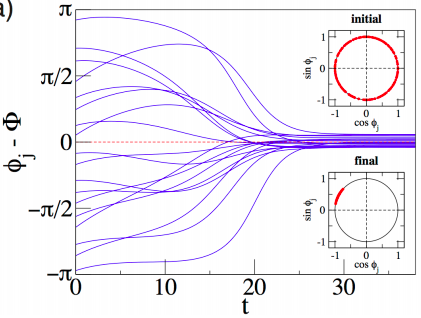
\includegraphics[width=0.5\textwidth]{kur100}
    \caption{
تحول زمانی فاز نوسانگرهای کوراموتو. در این شبیه‌سازی از ۱۰۰ نوسانگر استفاده شده است که فقط تحول زمانی فازهای ۱۸ عدد از نوسانگرها نمایش داده شده است. فرکانس ذاتی نوسانگرها به صورت تصادفی از توزیع نرمال (
$\mu=1.0$  و $\sigma=0.1$
) و فاز اولیه نوسانگرها نیز به صورت تصادفی از توزیع یکنواخت در بازه 
$[0,2\pi)$
انتخاب شده است. برای انتگرال‌گیری از روش اویلر با گام 
$dt\approx 0.01$
استفاده کرده‌ایم. واضح است که بعد از گذشت زمان همگامی نوسانگرها بیشتر شده است.
    }
    \label{fig:kur100-synch}
\end{figure}


\subsection{تابع پاسخ فاز}
با اعمال اختلال به یک نوسانگر و اندازه‌گیری اثر آن روی طول دوره نوسان می‌توان نمودار پاسخ فاز
\LTRfootnote{Phase Response Curve (PRC)}
 نوسانگر را بدست آورد. با توجه به شکل
 \ref{fig:prc}
پاسخ فاز نوسانگر را به صورت زیر تعریف می کنند:
\begin{equation}
\Delta \phi = (T_0 - T_1)/T_0
\label{eq:prc}
\end{equation}

\begin{figure}[h!]
	\centering
	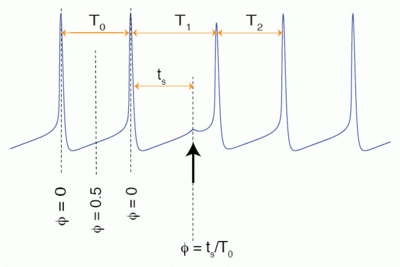
\includegraphics[width=0.5\textwidth]{prc}
    \caption{
با اعمال اختلال به یک نوسانگر و اندازه‌گیری اثر آن روی طول دوره نوسان می‌توان نمودار پاسخ فاز نوسانگر را بدست آورد.
\label{fig:prc}
    }
%    \label{fig:dbs-protocols}
\end{figure}

  نورون‌ها بر اساس تابع پاسخ فاز به دو دسته تقسیم می‌شوند. در نوع اول، با وارد کردن اختلال در هر لحظه‌ای فاز جلو می‌افتد؛ اما در نوع دوم، بر اساس لحظه اعمال اختلال فاز ممکن است جلو یا عقب بیفتد. نمودار پاسخ فاز این دو دسته در شکل 
\ref{fig:prc-type}
  نشان داده شده است.
  
\begin{figure}
	\centering
	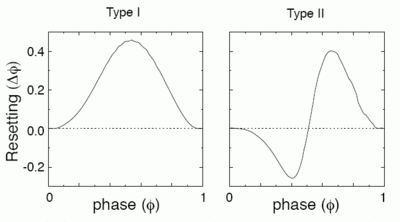
\includegraphics[width=0.5\textwidth]{prc-types}
    \caption{
  نورون‌ها بر اساس تابع پاسخ فاز به دو دسته تقسیم می‌شوند. در نوع اول، با وارد کردن اختلال در هر لحظه‌ای فاز جلو می‌افتد؛ اما در نوع دوم، بر اساس لحظه اعمال اختلال فاز ممکن است جلو یا عقب بیفتد.
    }
    \label{fig:prc-type}
\end{figure}

  
  
  
  
  
  
  
  
  
  
  
  
  
  
  
  
  
  
  
  
  
  